\chapter{Rendimiento observado de los alumnos}
\addcontentsline{toc}{chapter}{Rendimiento observado de los alumnos}

\section{Calificaciones obtenidas (Achiever)}

La primera medida de rendimiento que tendremos en cuenta son las calificaciones de los grupos de prácticas. Hay que tener en cuenta que estas calificaciones no son la evaluación final de cada grupo, sino la nota de la práctica cuya evolución se está analizando. Esta es la parte más subjetiva de la evaluación del rendimiento de cada alumno pues implica la participación del profesor y la toma en consideración de otros factores, además de los registrados en el servidor como puede ser la calidad de la memoria de la práctica. Las calificaciones muestran una distribución normal a lo largo de estos siete años de registros, ligeramente inclinada a la derecha porque las notas medias de esta asignatura suelen ser altas tal y como puede verse en la Figura \ref{fig:densityplotachiever}.

\begin{figure}[H]
    \centering
    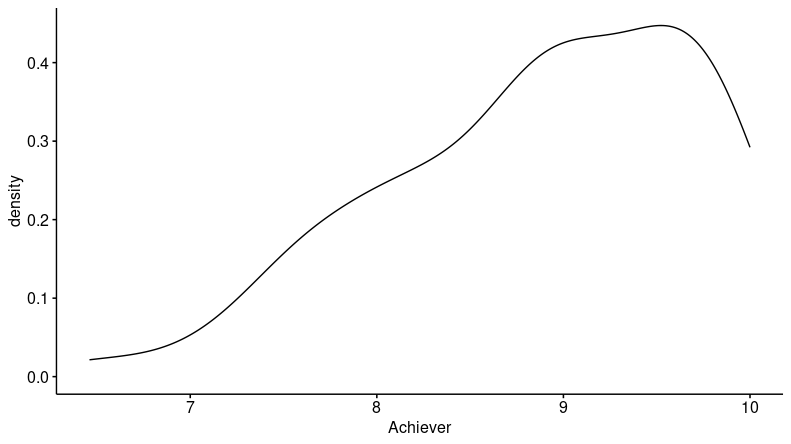
\includegraphics[width=0.85\textwidth]{NormalityAchiever5.png}
    \caption{Función de densidad de probabilidad de las calificaciones obtenidas por los distintos grupos de prácticas.}
    \label{fig:densityplotachiever}
\end{figure}

Además, la media está bastante balanceada (Figuras \ref{fig:boxplotresidualsachiever} y \ref{fig:histogramresidualsachiever}).

\begin{figure}[H]
\centering
\subfloat[Boxplot de los residuos de las calificaciones.]{\label{fig:boxplotresidualsachiever}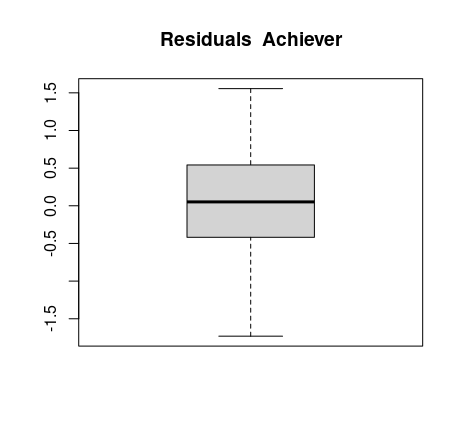
\includegraphics[width=0.47\textwidth]{NormalityAchiever3.png}}\qquad
\subfloat[Histograma de los residuos de las calificaciones.]{\label{fig:histogramresidualsachiever}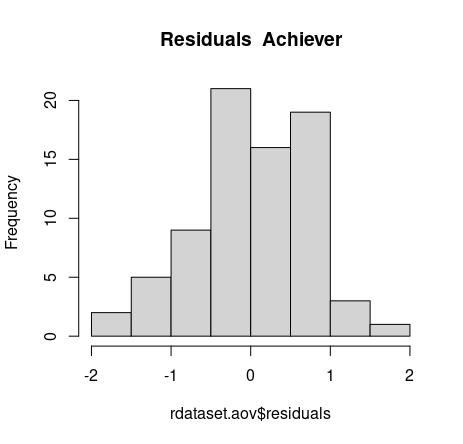
\includegraphics[width=0.47\textwidth]{NormalityAchiever4.png}}
\caption{Distribución de los residuos de las calificaciones.}
\label{fig:achiever}
\end{figure}

Además, la regresión es muy aceptable (Figura \ref{fig:q-qsessionsachiever}).

\begin{figure}[H]
    \centering
    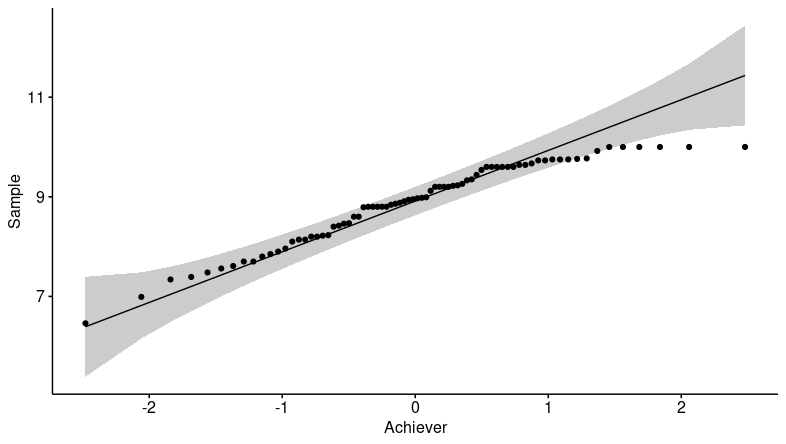
\includegraphics[width=0.75\textwidth]{NormalityAchiever6.png}
    \caption{Gráfico Q-Q de las calificaciones.}
    \label{fig:q-qsessionsachiever}
\end{figure}

A continuación se realizará un estudio por años de las calificaciones obtenidas. El boxplot de las calificaciones por años puede verse en la Figura \ref{fig:boxplotachieveryear}. Como puede verse, los datos recogidos muestran una variación muy perceptible en las notas a lo largo de los años. De hecho, los test estadísticos ratifican que hay diferentes significativas entre ellas. Tras realizar el test ANOVA de un factor (resultados en la Tabla \ref{tab:ANOVAachiever}) obtenemos $p = 0.0008 < 0.05$. Un análisis posterior por pares de Tukey muestra las diferencias entre los años (resultados en la Tabla \ref{tab:Tukeyachiever}). Podemos ver que el año 2017 es el principal elemento de disrupción, pero por poco margen. Lo mismo indica el análisis de los intervalos de confianza de la Figura \ref{fig:confidenceachiever}.

\begin{figure}[H]
    \centering
    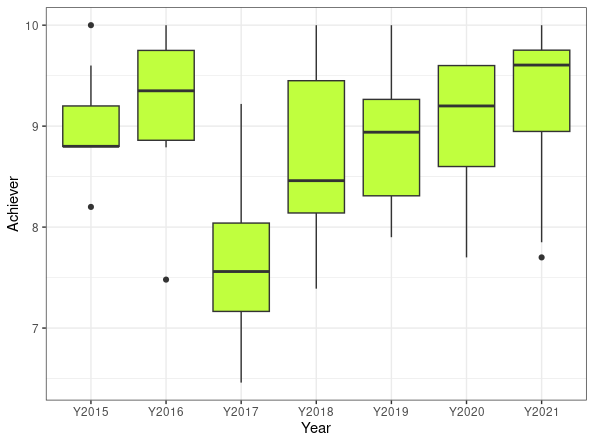
\includegraphics[width=0.6\textwidth]{boxplotachieveryear.png}
    \caption{Boxplot de las calificaciones por año.}
    \label{fig:boxplotachieveryear}
\end{figure}

% latex table generated in R 4.3.0 by xtable 1.8-4 package
% Sun Jun  4 18:14:08 2023
\begin{table}[H]
\centering
\caption{Resultados del test ANOVA de un solo factor (calificaciones).}
\label{tab:ANOVAachiever}
% latex table generated in R 4.3.0 by xtable 1.8-4 package
% Mon Jun  5 21:06:19 2023
\centering
\begin{tabular}{lrrrrr}
  \hline
 & Df & Sum Sq & Mean Sq & F value & Pr($>$F) \\ 
  \hline
rdataset[[Variable]] & 6 & 14.18 & 2.36 & 4.37 & 0.0008 \\ 
  Residuals            & 69 & 37.29 & 0.54 &  &  \\ 
   \hline
\end{tabular}
\end{table}

% latex table generated in R 4.3.0 by xtable 1.8-4 package
% Sun Jun  4 18:14:38 2023
\begin{table}[H]
\centering
\caption{Test HSD de Tukey (Honestly-significance-difference) de las calificaciones por años.}
\label{tab:Tukeyachiever}
\begin{tabular}{rrrrr}
  \hline
 & diff & lwr & upr & p adj \\ 
  \hline
Y2016-Y2015 & 0.18 & -0.88 & 1.23 & 1.00 \\ 
  \textbf{Y2017-Y2015} & -1.37 & -2.50 & -0.25 & 0.01 \\ 
  Y2018-Y2015 & -0.32 & -1.32 & 0.68 & 0.96 \\ 
  Y2019-Y2015 & -0.21 & -1.21 & 0.80 & 1.00 \\ 
  Y2020-Y2015 & -0.10 & -1.07 & 0.86 & 1.00 \\ 
  Y2021-Y2015 & 0.22 & -0.71 & 1.15 & 0.99 \\ 
  \textbf{Y2017-Y2016} & -1.55 & -2.67 & -0.42 & 0.00 \\ 
  Y2018-Y2016 & -0.50 & -1.50 & 0.51 & 0.74 \\ 
  Y2019-Y2016 & -0.38 & -1.39 & 0.62 & 0.91 \\ 
  Y2020-Y2016 & -0.28 & -1.25 & 0.69 & 0.97 \\ 
  Y2021-Y2016 & 0.05 & -0.89 & 0.98 & 1.00 \\ 
  \textbf{Y2018-Y2017} & 1.05 & -0.03 & 2.13 & 0.06 \\ 
  \textbf{Y2019-Y2017} & 1.16 & 0.08 & 2.24 & 0.03 \\ 
  \textbf{Y2020-Y2017} & 1.27 & 0.22 & 2.31 & 0.01 \\ 
  \textbf{Y2021-Y2017} & 1.59 & 0.58 & 2.60 & 0.00 \\ 
  Y2019-Y2018 & 0.11 & -0.84 & 1.06 & 1.00 \\ 
  Y2020-Y2018 & 0.22 & -0.70 & 1.13 & 0.99 \\ 
  Y2021-Y2018 & 0.54 & -0.33 & 1.42 & 0.50 \\ 
  Y2020-Y2019 & 0.10 & -0.81 & 1.02 & 1.00 \\ 
  Y2021-Y2019 & 0.43 & -0.45 & 1.30 & 0.75 \\ 
  Y2021-Y2020 & 0.33 & -0.51 & 1.16 & 0.90 \\ 
   \hline
\end{tabular}
\end{table}

\begin{figure}[H]
    \centering
    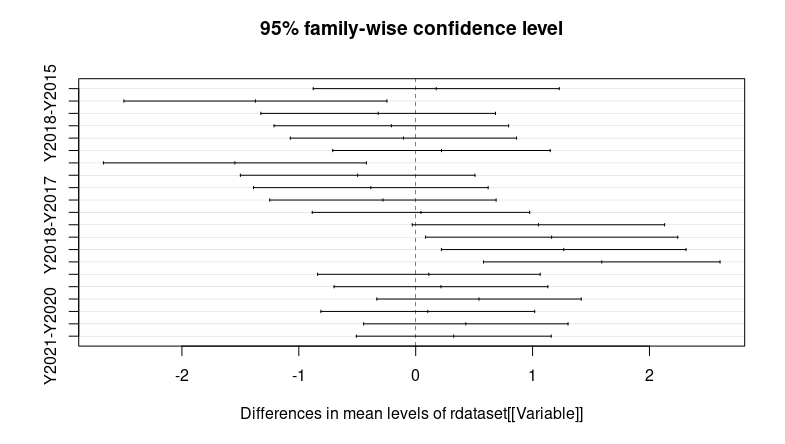
\includegraphics[width=0.80\textwidth]{NormalityAchiever1.png}
    \caption{Intervalos de confianza de las calificaciones por años.}
    \label{fig:confidenceachiever}
\end{figure}

\section{Número de sesiones realiazadas (Perseverant)}

Número de sesiones realizadas. También se ha visto antes.

\section{Número de intentos para resolver cada problema (SessionsBefore)}

Número de intentos: Número de veces que se abre un mismo problema sin resolver hasta que se resuelve por primera vez. Este valor está directamente relacionado con la tasa de fallo analizada anteriormente

\section{Sesiones perdidas durante un problema}

Con frecuencia ocurre que los alumnos, cuando intentan resolver un problema y no lo consiguen, saltan, curiosamente, a sesiones en otros problemas más complejos, los cuales, obviamente, tampoco pueden resolver.

\textbf{Falta gráfica.}

Este hábito es más frecuente de lo que parece y mantiene mucha variación en cada problema, sobre todo es más fuerte al comienzo de las prácticas, pero es homogéneo año tras año (ANOVA p=0.746, KW p=0.9) y se puede decir que está presente en la mayoría de los grupos. Aunque la mediana sea 0, casi todos los grupos (80\%) exhiben este comportamiento en algún momento.

\textbf{Referenciar tabla ya existente}.

\textbf{Falta gráfica.}

\section{Abrir un problema por primera vez (Newcomer)}

Momento exacto en el que se consigue abrir cada problema por primera vez en el servidor, normalizado para poder compararlo (normalizado porque cada año ha durado  un tiempo diferente)

\section{Resolver un problema por primera vez (EarlyBird)}

Momento exacto en el que se consigue resolver cada problema por primera vez, normalizado para poder compararlo (normalizado porque cada año ha durado  un tiempo diferente)

\textbf{Falta boxplot.}

Parece que, aunque los problemas están ordenados en orden creciente de dificultad, no siempre se resuelven en el mismo orden que se espera (ANOVA p=6.01e-7, KW p=1.18e-6), es decir P1 P2 P3 P4 P5 P6 P7 P8 P9. De hecho, se ha analizado este patrón y se han encontrado las siguientes variaciones en el que la más frecuente es la esperada por el profesor.

\section{Número total de problemas resueltos (Performer)}

Podemos observar que ha habido variaciones perceptibles durante los distintos años, con un caso especial en 2018 en el que hubo muchos grupos que no resolvieron todos los problemas (Figura \ref{fig:boxplotperformer}).

\begin{figure}[H]
    \centering
    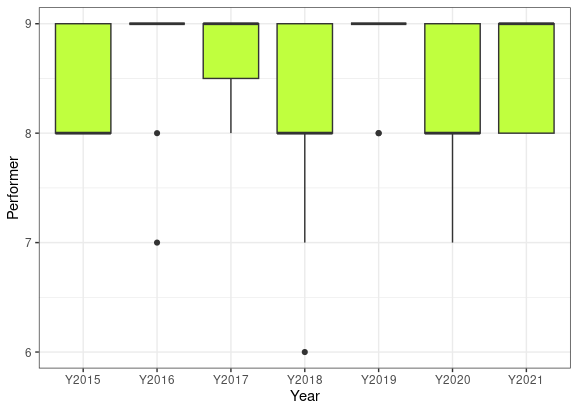
\includegraphics[width=0.6\textwidth]{boxplotperformer.png}
    \caption{Boxplot del número de problemas resueltos por año.}
    \label{fig:boxplotperformer}
\end{figure}

Sin embargo, las diferencias entre las medias no son estadísticamente significativas (considerando un nivel de significancia de $0.05$) tal y como puede verse en la Tabla \ref{tab:ANOVAperformer}.

Además, realizando un test de Tukey por pares de años (Tabla \ref{tab:Tukeyperformer}) se observa que todos los pares pueden considerarse estadísticamente iguales. La Figura \ref{fig:confidenceperformer} muestra los intervalos de confianza de todas las diferencias entre las distintas parejas de años.

% latex table generated in R 4.3.0 by xtable 1.8-4 package
% Tue Jun  6 20:27:28 2023
\begin{table}[H]
\centering
\caption{Resultados del test ANOVA de un solo factor (número de problemas resueltos).}
\label{tab:ANOVAperformer}
\begin{tabular}{lrrrrr}
  \hline
 & Df & Sum Sq & Mean Sq & F value & Pr($>$F) \\ 
  \hline
rdataset[[Variable]] & 6 & 4.63 & 0.77 & 1.76 & 0.1214 \\ 
  Residuals            & 69 & 30.37 & 0.44 &  &  \\ 
   \hline
\end{tabular}
\end{table}

% latex table generated in R 4.3.0 by xtable 1.8-4 package
% Tue Jun  6 20:27:48 2023
\begin{table}[ht]
\centering
\caption{Test HSD de Tukey (Honestly-significance-difference) del número de problemas resueltos por año.}
\label{tab:Tukeyperformer}
\begin{tabular}{rrrrr}
  \hline
 & diff & lwr & upr & p adj \\ 
  \hline
Y2016-Y2015 & 0.22 & -0.73 & 1.17 & 0.99 \\ 
  Y2017-Y2015 & 0.27 & -0.75 & 1.29 & 0.98 \\ 
  Y2018-Y2015 & -0.26 & -1.17 & 0.64 & 0.97 \\ 
  Y2019-Y2015 & 0.37 & -0.53 & 1.28 & 0.87 \\ 
  Y2020-Y2015 & -0.29 & -1.16 & 0.58 & 0.95 \\ 
  Y2021-Y2015 & 0.18 & -0.66 & 1.02 & 0.99 \\ 
  Y2017-Y2016 & 0.05 & -0.97 & 1.06 & 1.00 \\ 
  Y2018-Y2016 & -0.48 & -1.39 & 0.42 & 0.67 \\ 
  Y2019-Y2016 & 0.15 & -0.75 & 1.06 & 1.00 \\ 
  Y2020-Y2016 & -0.51 & -1.39 & 0.36 & 0.56 \\ 
  Y2021-Y2016 & -0.04 & -0.88 & 0.80 & 1.00 \\ 
  Y2018-Y2017 & -0.53 & -1.51 & 0.44 & 0.64 \\ 
  Y2019-Y2017 & 0.10 & -0.87 & 1.08 & 1.00 \\ 
  Y2020-Y2017 & -0.56 & -1.50 & 0.38 & 0.55 \\ 
  Y2021-Y2017 & -0.09 & -1.00 & 0.82 & 1.00 \\ 
  Y2019-Y2018 & 0.64 & -0.22 & 1.50 & 0.28 \\ 
  Y2020-Y2018 & -0.03 & -0.85 & 0.80 & 1.00 \\ 
  Y2021-Y2018 & 0.44 & -0.35 & 1.23 & 0.61 \\ 
  Y2020-Y2019 & -0.66 & -1.49 & 0.16 & 0.20 \\ 
  Y2021-Y2019 & -0.19 & -0.98 & 0.60 & 0.99 \\ 
  Y2021-Y2020 & 0.47 & -0.28 & 1.22 & 0.49 \\ 
   \hline
\end{tabular}
\end{table}

\begin{figure}[H]
    \centering
    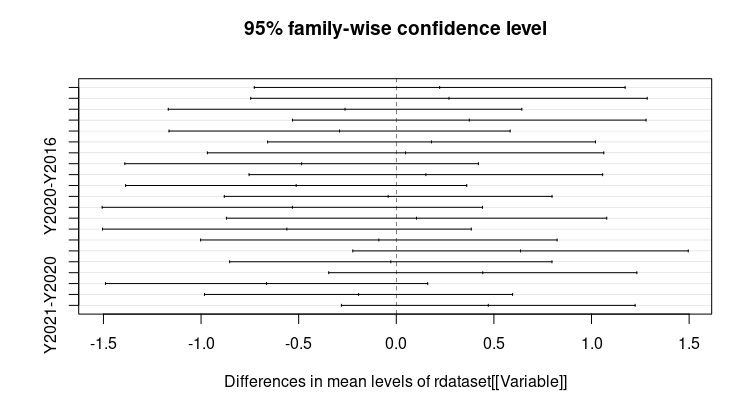
\includegraphics[width=0.80\textwidth]{NormalityPerformer1.png}
    \caption{Intervalos de confianza del número de problemas resueltos por año.}
    \label{fig:confidenceperformer}
\end{figure}

\section{Siguiendo el plan del profesor (Follower)}

Se incorpora una medida de similaridad Follower en [0,1] que cuantifica cómo se parece el patrón encontrado con respecto al patrón esperado. \textbf{Falta footnote.}

\textbf{Falta tabla.}